% This is an example of a latex file for an assignment in
% a university math class
%
%------------------------------------------------------------
%---------------- A S S I G N M E N T - 1 -------------------
%------------------------------------------------------------
\documentclass[a4paper,12pt,addpoints]{exam}
\usepackage{graphicx}
\usepackage[usenames,svgnames]{xcolor}
\usepackage{wrapfig}
\usepackage{hyperref}
\usepackage{multicol,booktabs,enumitem}
\usepackage{siunitx,textcomp}%for the degree symbol: The angle is \ang{30}.
\usepackage{amsmath,amssymb}
\usepackage{pgfplots}
\pgfplotsset{colormap/blackwhite}
\usepgfplotslibrary{fillbetween}
\usepackage{hyperref}
\hypersetup{
	colorlinks,
	linkcolor={blue!50!black},
	urlcolor={blue!50!black}
}
\usepackage{tasks}
% solution shortcuts
\newcommand{\Desmos}{\href{http://www.desmos.com/calculator}{\texttt{Desmos\,}}}%
\newcommand{\bp}{\begin{parts}}
\newcommand{\ep}{\end{parts}}
\newcommand{\bs}{\begin{solution}}
\newcommand{\es}{\end{solution}}
%--------------------------------------------------
% solution formatting
\pointpoints{mark}{marks}
% no header on page 1
\thispagestyle{empty}
% when 'answers' is added to the document class, the solutions are
% printed without a box. Comment this to box the solutions.
\pointpoints{mark}{marks}%
\unframedsolutions%
\SolutionEmphasis{\color{Navy}}
%---------------------------------------------------
\lhead{ENGE401}
\ifprintanswers
	\rhead{Assignment 1 -- \textcolor{DeepPink}{\textbf{SOLUTIONS}}}
\else
	\rhead{Assignment 1}
\fi
%---------------------------------------------------
\begin{document}

%\partialgradetable{1-8}[v][questions]
\begin{center}
\vspace{0.25cm}
\large{School of Engineering, Computer \& Mathematical Sciences}\\

\ifprintanswers
	\large{\textcolor{DeepPink}{\textbf{SOLUTIONS}}}
\fi
\end{center}
\begin{center}
	%\vspace{0.5cm}
	\hypersetup{linkcolor={black}}
	\cellwidth{1.7em}
	\gradetable[h][questions]
	\vspace{0.5cm}
\end{center}
\begin{questions}
%%%%%%%%%%%%%%%%%%%%%%%%%%%%%%%%%%%%%%%%%%%%
%%%%%%%%%%%% Q U E S T I O N %%%%%%%%%%%%%%%
%%%%%%%%%%%%%%%%%%%%%%%%%%%%%%%%%%%%%%%%%%%%

	\question Think about the course title: Engineering Mathematics. In a few sentences answer the\\ following:
		\bp
		\part[1] What is mathematics?
			\bs Mathematics is a language used to communicate rules of logic.\es

		\part[1] What is engineering?
			\bs Engineering is the application of science to society. Science is studied using the framework of logic which is communicated through mathematics. A paper in engineering mathematics covers foundations in mathematics that can enable you to apply scientific knowledge to solve problems in society.\es
		\ep


%%%%%%%%%%%%%%%%%%%%%%%%%%%%%%%%%%%%%%%%%%%%
%%%%%%%%%%%% Q U E S T I O N %%%%%%%%%%%%%%%
%%%%%%%%%%%%%%%%%%%%%%%%%%%%%%%%%%%%%%%%%%%%

\question The distance an object falls when dropped from rest can be calculated using the formula:
\[\Delta x=\frac{1}{2}at^2\]
where $a=9.8$ ms$^{-2}$ is the acceleration due to gravity and $t$ is time in seconds.
\bp\part[4] Find stuff here.\ep

%%%%%%%%%%%%%%%%%%%%%%%%%%%%%%%%%%%%%%%%%%%%
%%%%%%%%%%%% Q U E S T I O N %%%%%%%%%%%%%%%
%%%%%%%%%%%%%%%%%%%%%%%%%%%%%%%%%%%%%%%%%%%%

		\question \bp\part[4] Find the points of intersection of the two functions:
\[\left(\frac{x}{2}\right)^2+y^2=25\tag{1}\]
\[x^2-2y=8\tag{2}\]
		\bs
		From equation (2) isolate $x^2=8+2y$ and sub into equation (1):
		\begin{align*}
		\frac{x^2}{4}+y^2&=25\\
		\frac{8+2y}{4}+y^2&=25\\
		y^2+\frac{y}{2}-23&=0\\
		2y^2+y-46&=0
	\end{align*}
Use the quadratic formula to solve for $y$:
\begin{align*}
y&=\frac{-1\pm \sqrt{1^2-4(2)(-46)}}{2(2)}\\
y&=\frac{-1\pm \sqrt{369}}{4}\\
		y_1&=4.55 \mbox{ or }y_2=-5.05\\
		\end{align*}
		Sub $y$-values in to find the $x$-values:\\\medskip
		Using $y_1=4.55$, then $x_1=\sqrt{8+2(4.55)}=\pm4.13$\\
		Using $y_2=-5.05$, then $x_2=\sqrt{-2.1}$, which has no solution because the square root of negative numbers does not exist in $\mathbb{R}$.

		Therefore, the points of intersection are $(4.13,4.55)$, and $(-4.13,4.55)$.
		\es
		\part[4] Include a \Desmos plot with your submission. Show the points of intersection on the plot.

		\begin{center}
			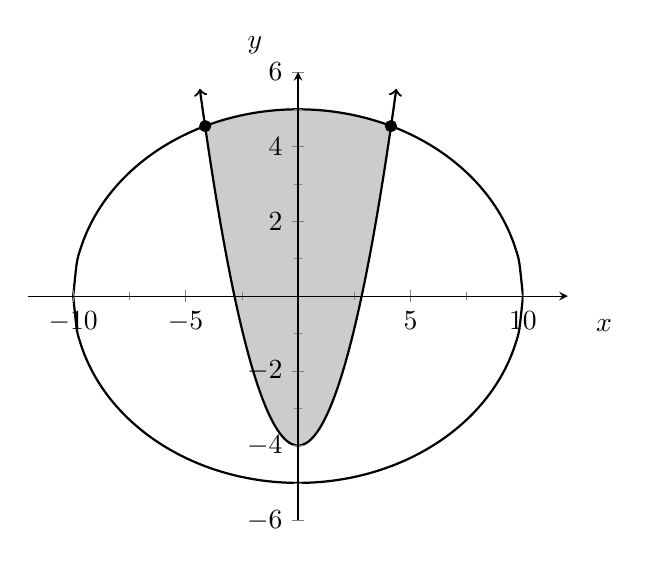
\begin{tikzpicture}
			\begin{axis}[%grid=both,
			axis on top=true,
			%scale=1,
			%unit vector ratio=1 1,
			ymin=-6,ymax=6,
			xmin=-12,xmax=12,
			minor tick num=1,
			axis lines = middle,
			xlabel=$x$,
			ylabel=$y$,
			label style ={at={(ticklabel cs:1.1)}}
			]
			\addplot[<->,domain=-4.37:4.37,samples=100,smooth,thick,black,name path=parab] {0.5*x^2-4};
			\addplot[-,domain=-10:10,samples=125,smooth,thick,black,name path=ellipseP] {sqrt(25-0.25*x^2)};
			\addplot[-,domain=-10:10,samples=125,smooth,thick,black,name path=ellipseN] {-sqrt(25-0.25*x^2)};
			\addplot[gray!40]fill between[of=ellipseP and parab,soft clip={domain=-4.136:4.136}];
			\addplot[mark=*] coordinates {(4.13,4.55)};
			\addplot[mark=*] coordinates {(-4.13,4.55)};
			\end{axis}
			\end{tikzpicture}
		\end{center}

\ep


%%%%%%%%%%%%%%%%%%%%%%%%%%%%%%%%%%%%%%%%%%%%
%%%%%%%%%%%% Q U E S T I O N %%%%%%%%%%%%%%%
%%%%%%%%%%%%%%%%%%%%%%%%%%%%%%%%%%%%%%%%%%%%

\question Given the sine function $$\displaystyle 2y=2\sin\left(2\left(x+\frac{\pi}{4}\right)\right)$$
\bp
\part[2] Find the amplitude, period in radians, phase shift, and vertical shift.

\part[4] Plot the function using \Desmos on the restricted domain: ${-\frac{3\pi}{2}\le x \le \frac{3\pi}{2}}$. \ep

%%%%%%%%%%%%%%%%%%%%%%%%%%%%%%%%%%%%%%%%%%%%
%%%%%%%%%%%% Q U E S T I O N %%%%%%%%%%%%%%%
%%%%%%%%%%%%%%%%%%%%%%%%%%%%%%%%%%%%%%%%%%%%

\bonusquestion[4] Use a graphics package such as \Desmos to plot your initials. Your plot must contain (at least):
\begin{itemize}
	\item two characters (any language)
	\item one curved section (e.g., circular, quadratic, sine, cosine etc.)
	\item one shaded region (e.g., $x<5$; $f(x)>\sin x$ etc.)
	\item a list of the functions plotted
\end{itemize}
Include a printout or screenshot of your design with your submission.
\end{questions}
\end{document}
%---------------------------------------------------------
% //end assignment
% Have a good day :-)
% -Jeff---------------------------------------------------
